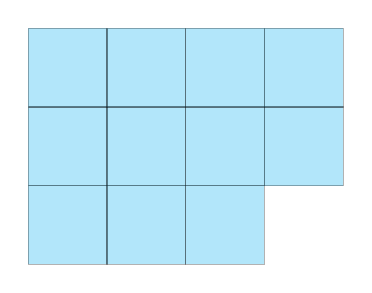
\begin{tikzpicture}
    \coordinate (A) at (0,0);
    \coordinate (B) at (2,0);
    \coordinate (C) at (2,1);
    \coordinate (D) at (0,1);
    \coordinate (E) at (0,3);
    \coordinate (F) at (2,3);
    \coordinate (G) at (4,3);
    \coordinate (H) at (4,1);
    \coordinate (I) at (3,0);
    \coordinate (J) at (3,1);
    \coordinate (K) at (1,0);
    \coordinate (L) at (1,1);
    \coordinate (M) at (0,2);
    \coordinate (N) at (1,2);
    \coordinate (O) at (2,2);
    \coordinate (P) at (3,2);
    \coordinate (Q) at (4,2);
    \coordinate (R) at (1,3);
    \coordinate (S) at (3,3);

    \draw[fill=cyan,thin,opacity=0.3] (A) -- (K) -- (L) -- (D) --cycle;
    \draw[fill=cyan,thin,opacity=0.3] (K) -- (B) -- (C) -- (L) --cycle;
    \draw[fill=cyan,thin,opacity=0.3] (B) -- (I) -- (J) -- (C) --cycle;
    \draw[fill=cyan,thin,opacity=0.3] (D) -- (L) -- (N) -- (M) --cycle;
    \draw[fill=cyan,thin,opacity=0.3] (L) -- (C) -- (O) -- (N) --cycle;
    \draw[fill=cyan,thin,opacity=0.3] (C) -- (J) -- (P) -- (O) --cycle;
    \draw[fill=cyan,thin,opacity=0.3] (J) -- (H) -- (Q) -- (P) --cycle;
    \draw[fill=cyan,thin,opacity=0.3] (M) -- (N) -- (R) -- (E) --cycle;
    \draw[fill=cyan,thin,opacity=0.3] (N) -- (O) -- (F) -- (R) --cycle;
    \draw[fill=cyan,thin,opacity=0.3] (O) -- (P) -- (S) -- (F) --cycle;
    \draw[fill=cyan,thin,opacity=0.3] (P) -- (Q) -- (G) -- (S) --cycle;
\end{tikzpicture}